\documentclass[11pt]{article}

\usepackage{tikz}
\usetikzlibrary{automata,positioning}

\begin{document}

\clearpage
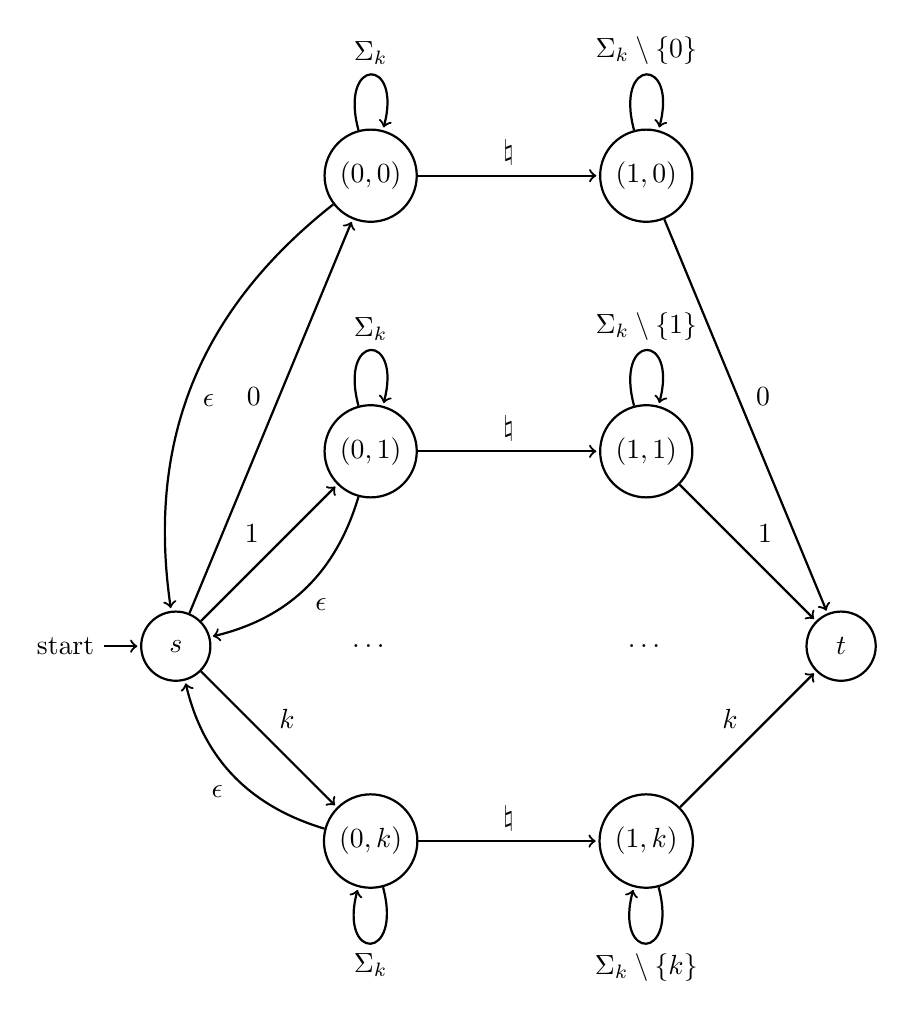
\begin{tikzpicture}[->,shorten >=1pt, auto, on grid, node distance=3.5cm, thick, node/.style={circle,draw}]
	\node[state,initial] (qs) {$s$};
	\node[state] (q1) [above right=of qs] {$(0,1)$};
	\node[state] (q0) [above=of q1] {$(0,0)$};
	\node[state] (qk) [below right=of qs] {$(0,k)$};
	\node[state] (qq0)[right=of q0] {$(1,0)$};
	\node[state] (qq1)[right=of q1] {$(1,1)$};
	\node[state] (qqk)[right=of qk] {$(1,k)$};
	\node[state] (t)  [above right=of qqk] {$t$};
	\path (qs) edge node {0} (q0);
	\path (qs) edge node {1} (q1);
	\path (qs) edge node {$k$} (qk);
	\path (q0) edge[bend right] node {$\epsilon$} (qs);
	\path (q1) edge[bend left] node {$\epsilon$} (qs);
	\path (qk) edge[bend left] node {$\epsilon$} (qs);
	\path (q1) -- node[auto=false]{\ldots} (qk);
	\path (qq1) -- node[auto=false]{\ldots} (qqk);
	\path (q0) edge node {$\natural$} (qq0);
	\path (q1) edge node {$\natural$} (qq1);
	\path (qk) edge node {$\natural$} (qqk);
	\path (q0) edge [loop above] node {$\Sigma_k$} ();
	\path (q1) edge [loop above] node {$\Sigma_k$} ();
	\path (qk) edge [loop below] node {$\Sigma_k$} ();
	\path (qq0) edge [loop above] node {$\Sigma_k\setminus\{0\}$} ();
	\path (qq1) edge [loop above] node {$\Sigma_k\setminus\{1\}$} ();
	\path (qqk) edge [loop below] node {$\Sigma_k\setminus\{k\}$} ();
	\path (qq0) edge node {0} (t);
	\path (qq1) edge node {1} (t);
	\path (qqk) edge node {$k$} (t);
\end{tikzpicture}

\end{document}
